%杨舒云的实验报告编辑界面,使用了Huanyu Shi,2019级的模板,杨舒云在此拜谢ORZ!

%!TEX program = xelatex
\documentclass[dvipsnames, svgnames,a4paper,11pt]{article}
% ----------------------------------------------------- 
%	加边框的命令
%	参考:https://tex.stackexchange.com/questions/531559/how-to-add-the-page-border-for-first-two-pages-in-latex
\usepackage{tikz}
\usetikzlibrary{calc}
\usepackage{eso-pic}
\AddToShipoutPictureBG{%
\begin{tikzpicture}[overlay,remember picture]
\draw[line width=0.6pt] % 边框粗细
    ($ (current page.north west) + (0.6cm,-0.6cm) $)
    rectangle
    ($ (current page.south east) + (-0.6cm,0.6cm) $); % 边框位置
\end{tikzpicture}}


\usepackage{xcolor}
\definecolor{c1}{HTML}{086173} % 目录颜色 原版为2752C9 紫灰色535AAA 蓝紫色0B0DB7 深蓝色070F94 湖绿色219394 松石灰绿086173
\definecolor{c2}{HTML}{E20129} % 引用颜色 原版\definecolor{c2}{RGB}{190,20,83} 橙色F24729

\usepackage{ctex}
\usepackage[top=28mm,bottom=28mm,left=15mm,right=15mm]{geometry}
\usepackage{hyperref} 
\hypersetup{
	colorlinks,
	linktoc = section, % 超链接位置,选项有section, page, all
	linkcolor = c1, % linkcolor 目录颜色
	citecolor = c1  % citecolor 引用颜色
}
\usepackage{amsmath,enumerate,multirow,float}
\usepackage{tabularx}
\usepackage{tabu}
\usepackage{subfig}
\usepackage{fancyhdr}
\usepackage{graphicx}
\usepackage{wrapfig}  
\usepackage{physics}
\usepackage{appendix}
\usepackage{amsfonts}

%
\usepackage{tcolorbox}
\tcbuselibrary{skins,breakable}
\newtcolorbox{tbox}[2][]{
    colframe=black!70!,
    breakable,
    enhanced,
	boxrule =0.5pt,
    title = {#2},
    fonttitle = \large\kaishu\bfseries,
	drop fuzzy shadow,
    #1
}
\newtcolorbox[auto counter,number within=section]{question}[1][]{
  top=2pt,bottom=2pt,arc=1mm,
  boxrule=0.5pt,
%   frame hidden,
  breakable,
  enhanced, %跨页后不会显示下边框
  coltitle=c1!80!gray,
  colframe=c1,
  colback=c1!3!white,
  drop fuzzy shadow,
  title={思考题~\thetcbcounter:\quad},
  fonttitle=\bfseries,
  attach title to upper,
  #1
}

% ---------------------------------------------------------------------
%	利用cleveref改变引用格式,\cref是引用命令
\usepackage{cleveref}
\crefformat{figure}{#2{\textcolor{c2}{Figure #1}}#3} % 图片的引用格式
\crefformat{equation}{#2{(\textcolor{c2}{#1})}#3} % 公式的引用格式
\crefformat{table}{#2{\textcolor{c2}{Table #1}}#3} % 表格的引用格式


% ---------------------------------------------------------------------
%	页眉页脚设置
\fancypagestyle{plain}{\pagestyle{fancy}}
\pagestyle{fancy}
\lhead{\kaishu 中山大学物理与天文学院\uppercase\expandafter{\romannumeral1}} % 左边页眉,学院 + 课程
\rhead{\kaishu 杨舒云的实验报告} % 右边页眉,实验报告标题
\cfoot{\thepage} % 页脚,中间添加页码


% ---------------------------------------------------------------------
%	对目录、章节标题的设置
\renewcommand{\contentsname}{\centerline{\huge 目录}}
\usepackage{titlesec}
\usepackage{titletoc}
% \titleformat{章节}[形状]{格式}{标题序号}{序号与标题间距}{标题前命令}[标题后命令]
\titleformat{\section}{\centering\LARGE\songti}{}{1em}{}

% ---------------------------------------------------------------------
%   listing代码环境设置
\usepackage{listings}
\lstloadlanguages{python}
\lstdefinestyle{pythonstyle}{
backgroundcolor=\color{gray!5},
language=python,
frameround=tftt,
frame=shadowbox, 
keepspaces=true,
breaklines,
columns=spaceflexible,                   
basicstyle=\ttfamily\small, % 基本文本设置,字体为teletype,大小为scriptsize
keywordstyle=[1]\color{c1}\bfseries, 
keywordstyle=[2]\color{Red!70!black},   
stringstyle=\color{Purple},       
showstringspaces=false,
commentstyle=\ttfamily\scriptsize\color{green!40!black},%注释文本设置,字体为sf,大小为smaller
tabsize=2,
morekeywords={as},
morekeywords=[2]{np, plt, sp},
numbers=left, % 代码行数
numberstyle=\it\tiny\color{gray}, % 代码行数的数字字体设置
stepnumber=1,
rulesepcolor=\color{gray!30!white}
}




% ---------------------------------------------------------------------
%	其他设置
\def\degree{${}^{\circ}$} % 角度
\graphicspath{{./images/}} % 插入图片的相对路径
\allowdisplaybreaks[4]  %允许公式跨页 
\usepackage{lipsum}
\usepackage{adjustbox}
%\usepackage{mathrsfs} % 字体
\captionsetup[figure]{name=Figure} % 图片形式
\captionsetup[table]{name=Table} % 表格形式

\usepackage{enumitem}
\usepackage{tabularray}  %绘制表格时可以更加方便添加框线
\usepackage{xcolor} %添加更多文本颜色


%---------------------------------------------------------------------
%	正文
%---------------------------------------------------------------------


\begin{document}
	
	
	
	% 实验报告封面	
	
	% 顶栏
	\begin{table}
		\renewcommand\arraystretch{1.7}
		\begin{tabularx}{\textwidth}{
				|>{\centering}X|>{\centering}X|>{\centering}X
				|>{\centering}X|>{\centering}X|>{\centering\arraybackslash}X|}
			\hline
			\multicolumn{2}{|c|}{预习报告}&\multicolumn{2}{c|}{实验记录与分析}&\multicolumn{2}{c|}{总成绩}\\
			\hline
			\LARGE30 & & \LARGE50 & & \LARGE80 & \\
			\hline
		\end{tabularx}
	\end{table}
	% ---
	
	% 信息栏
	\begin{table}
		\renewcommand\arraystretch{1.7}
		\begin{tabularx}{\textwidth}{|X|X|X|X|}
			\hline
			年级、专业: & 2022级 物理学 &组号: & 实验班2\\
			\hline
			姓名: & 杨舒云  & 学号: & 22344020\\
			\hline
			实验时间: & 2024/3/25 & 教师签名: & \\
			\hline
		\end{tabularx}
	\end{table}
	% ---
	
	% 大标题
	\begin{center}
		\LARGE Lab2-4 \quad 光学像差实验I
	\end{center}
	% ---
	
	% 注意事项
	
	% 基本
	\textbf{【实验报告注意事项】}
	\begin{enumerate}[label=\arabic*., leftmargin=*]
		\item 实验报告由两部分组成:
		\begin{enumerate}[label=\arabic*), leftmargin=*]
			\item 预习报告:课前认真研读\textbf{实验讲义},弄清实验原理;实验所需的仪器设备、用具及其使用、完成课前预习思考题;了解实验需要测量的物理量,并根据要求提前准备实验记录表格(可以参考实验报告模板,可以打印)。\textcolor{red}{\textbf{(30分)}}
			\item 实验记录与分析:认真、客观记录实验条件、实验过程中的现象以及数据。实验记录请用珠笔或者钢笔书写并签名(\textcolor{red}{\textbf{用铅笔记录的被认为无效}})。\textcolor{red}{\textbf{保持原始记录,包括写错删除部分,如因误记需要修改记录,必须按规范修改。}}(不得手记的值输入到电脑打印);离开前请实验教师检查记录并签名。\textcolor{red}{\textbf{(50分)}}
		\end{enumerate}
		
		\item \textcolor{red}{\textbf{本实验报告可提前打印出来,当场记录分析完成交给带实验的老师,课后无需再提交。若当场完成不了,则请课后完成,再扫描并通过seelight提交。}}
		
		\textcolor{red}{\textbf{注意:本文档已留出填写空间,若填写空间不够的话请提前规划留白,做到报告的美观}}
		\item 注意事项:
		\begin{enumerate}[label=\arabic*), leftmargin=*]
			\item 实验中\textcolor{red}{\textbf{避免激光器伤到眼睛}}
			\item 避免用手直接接触镜片的光学面
			\item 安装镜片时需在光学平台上尽量靠近台面的高度操作,以免失手跌落摔碎镜片
			\item 实验平台配件所用固定螺钉需拧紧,以免镜架晃动;但不可过紧,以免损坏
			\item 实验前需按仪器清单检查光学元件是否齐全,\textcolor{red}{\textbf{实验结束后按照顺序放回元件盒}}
			
		\end{enumerate}
	\end{enumerate}
	
	% 安全
	\textbf{【实验安全注意事项】}	
	\begin{enumerate}
		\item 实验中需带手套,尽量避免用手直接接触镜片的光学面。若不小心触摸了光学表面,需尽快用镜头纸或擦镜布擦拭干净。
		\item 安装镜片时需在光学平台上尽量靠近台面的高度操作,以免失手跌落摔碎镜片。
		\item 实验平台配件所用固定螺钉需拧紧,以免镜架晃动;但不可过紧,以免损坏。
		\item 实验前需按仪器清单检查光学元件是否齐全,实验结束后按照顺序放回元件盒。
	\end{enumerate}	
	% ---
	
	% 特别鸣谢
	\textbf{【特别鸣谢及模板说明】}	
	
	感谢2019级学长石寰宇为本实验报告提供\LaTeX 模板。\textcolor{red}{\textbf{由于原实验报告模板缺少实验编号,为方便在电脑上整理,故添加自命名编号Lab2-4}}
	% ---
	
	
	
	% 目录
	\clearpage
	\tableofcontents
	\clearpage
	% ---
	
	
	
	% 预习报告	
	
	% 小标题
	\setcounter{section}{0}
	\section{Lab2-4 光学像差实验I \quad\heiti 预习报告}
	% ---
	
	% 实验目的
	\subsection{实验目的}
	\subsection{实验目的}
	\begin{enumerate}
		\item 了解七种几何像差产生的原理、基本规律;
		\item 了解各种像差对光学成像质量的影响;
		\item 掌握慧差、色差产生的原理及其测量表征; 
		\item 掌握光学系统的基本调试方法。
	\end{enumerate}
	% ---
	
	% 仪器用具
	\subsection{仪器用具}
	\begin{table}[htbp]
		\centering
		\begin{tabular}{|c|c|c|c|}
			\hline
			产品编号 & 产品名称 & 规格 & 数量 \\
			\hline
			1 & 激光光源 & $\lambda =632.6nm$ & 1 \\
			2 & 激光器夹持器 & 3维调整 & 1 \\
			3 & 显微物镜 & 10×/0.25 & 1 \\
			4 & 针孔 & Ø100um或Ø50um & 1 \\
			5 & 五维调整机构 & 装配显微物镜和针孔用 & 1 \\
			6 & 衰减片1 & 0.0001(衰减系数),装在镜框中 & 1 \\
			7 & 衰减片2 & 0.01(衰减系数),装在镜框中 & 1 \\
			8 & 双凸透镜1 & 焦距$f=300mm$,装在透镜/反射镜座中 & 1 \\
			9 & 平凸透镜2 & 焦距$f=100mm$,装在透镜/反射镜座中 & 1 \\
			10 & 平凸透镜3 & 焦距$f=150mm$,装在透镜/反射镜座中 & 1 \\
			11 & 白屏 & SZ-13,一面白屏,一面带坐标纸 & 1 \\
			12 & 成像相机 & 大恒的MER-130-30UM或元启智能的REV-13AMU2C & 1 \\
			13 & 数据线 & 图像采集数据线 & 1 \\
			14 & 计算机 & 台式或笔记本,安装有成像相机图像采集软件 & 1 \\
			15 & 光学导轨 & 长度1米,带刻度 & 1 \\
			16 & 二维平移台 & 行程>10mm & 4 \\
			17 & 平移滑块 & & 8 \\
			18 & 支杆 & 50mm长和75mm长 & 3+5 \\
			19 & 磁性表座 & & 4 \\
			20 & 旋转调整台 & 可调角度>±5° & 1 \\
			21 & 白光灯 & GY-6型,亮度可调,即溴钨灯 & 1 \\
			22 & 滤光片1 & 透光波长:435nm & 1 \\
			23 & 滤光片2 & 透光波长:630nm & 1 \\
			\hline
		\end{tabular}
	\end{table}
	% ---
	
	% 原理概述
	\subsection{原理概述}
	\begin{enumerate}
		\item \textbf{色差}
		
		色差产生的原理主要基于不同颜色(波长)的光在折射介质中的折射率不同这一物理现象。这种现象导致了在光学系统中,不同颜色的光束在经过折射或反射后聚焦于不同的位置,形成了位置色差和倍率色差两种主要类型的色差。
		
		\begin{figure}[htbp]
			\centering
			\subfloat[]{
				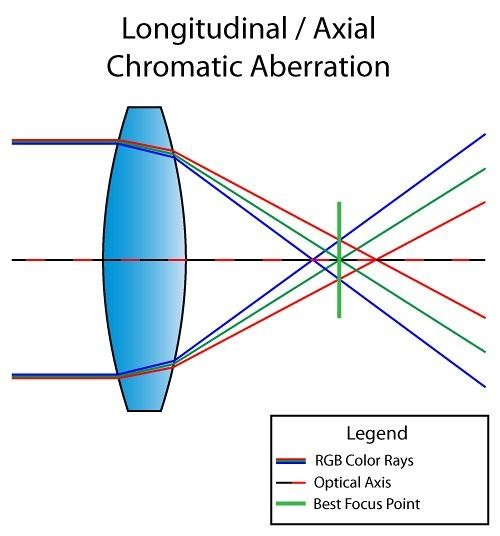
\includegraphics[width=0.3\textwidth]{Lab2_4Gra2.jpg}
			}
			\subfloat[]{
				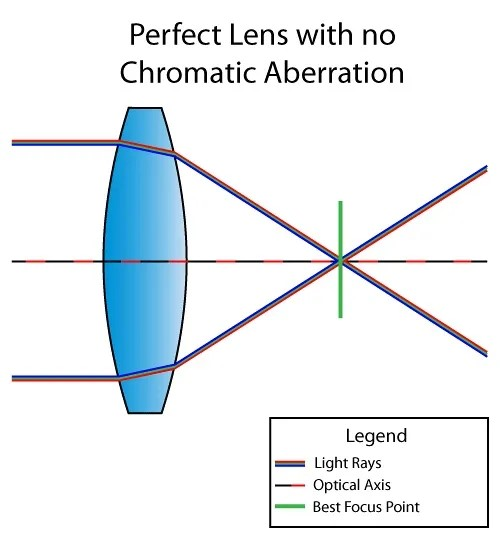
\includegraphics[width=0.3\textwidth]{Lab2_4Gra3.jpg}
			}
			\subfloat[]{
				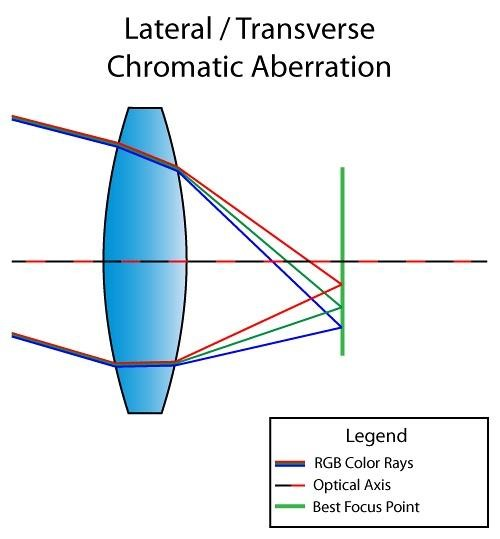
\includegraphics[width=0.3\textwidth]{Lab2_4Gra4.jpg}
			}
			\caption{光学色差}
			\label{fig:fig2}			
		\end{figure}
		
		\begin{itemize}
			\item \textbf{位置色差(轴向色差)} 主要是因为不同颜色的光束在通过光学系统后,其焦点与光轴的交点位置不同。这导致在任何给定的像面位置,物点的像是一个彩色的弥散斑,从而影响成像的清晰度和色彩的准确性。
			
			\item \textbf{倍率色差(横向色差或垂轴色差)} 则是因为光学系统对于不同颜色的光具有不同的垂轴放大率,导致同一个轴外物点的不同色光在像面上的大小(即图像的高度)不一致。
		\end{itemize}
		
		这两种色差的存在,尤其是在高精度的成像需求中,都必须通过光学设计的优化或使用特殊的光学材料和元件(如非球面透镜、复合透镜等)来进行校正和消除。		
		
		\item \textbf{慧差}
		
		\textbf{慧差的产生原理}
		
		慧差(也称为彗差或彗形像差)是当光学系统不满足等晕条件时产生的一种像差,主要发生在轴外光束上。在这种情况下,近轴点成像光束的对称性被破坏,导致原本应该在像方对称主光线的各个光线交点不再位于主光线上。这种失对称的像差会使成像光束与高斯像面相交,形成一个类似彗星尾巴状的弥散斑。
		
		慧差的产生与光束通过光学系统的孔径大小和视场位置有关,它既与孔径相关,也与视场相关。慧差的存在会使轴外的像点变成彗星状的弥散斑,严重影响轴外像点的清晰程度。在设计光学系统时,通过适当的设计和调整可以减小或消除慧差的影响,从而提高成像质量。
		
		\begin{figure}[htbp]
			\centering
			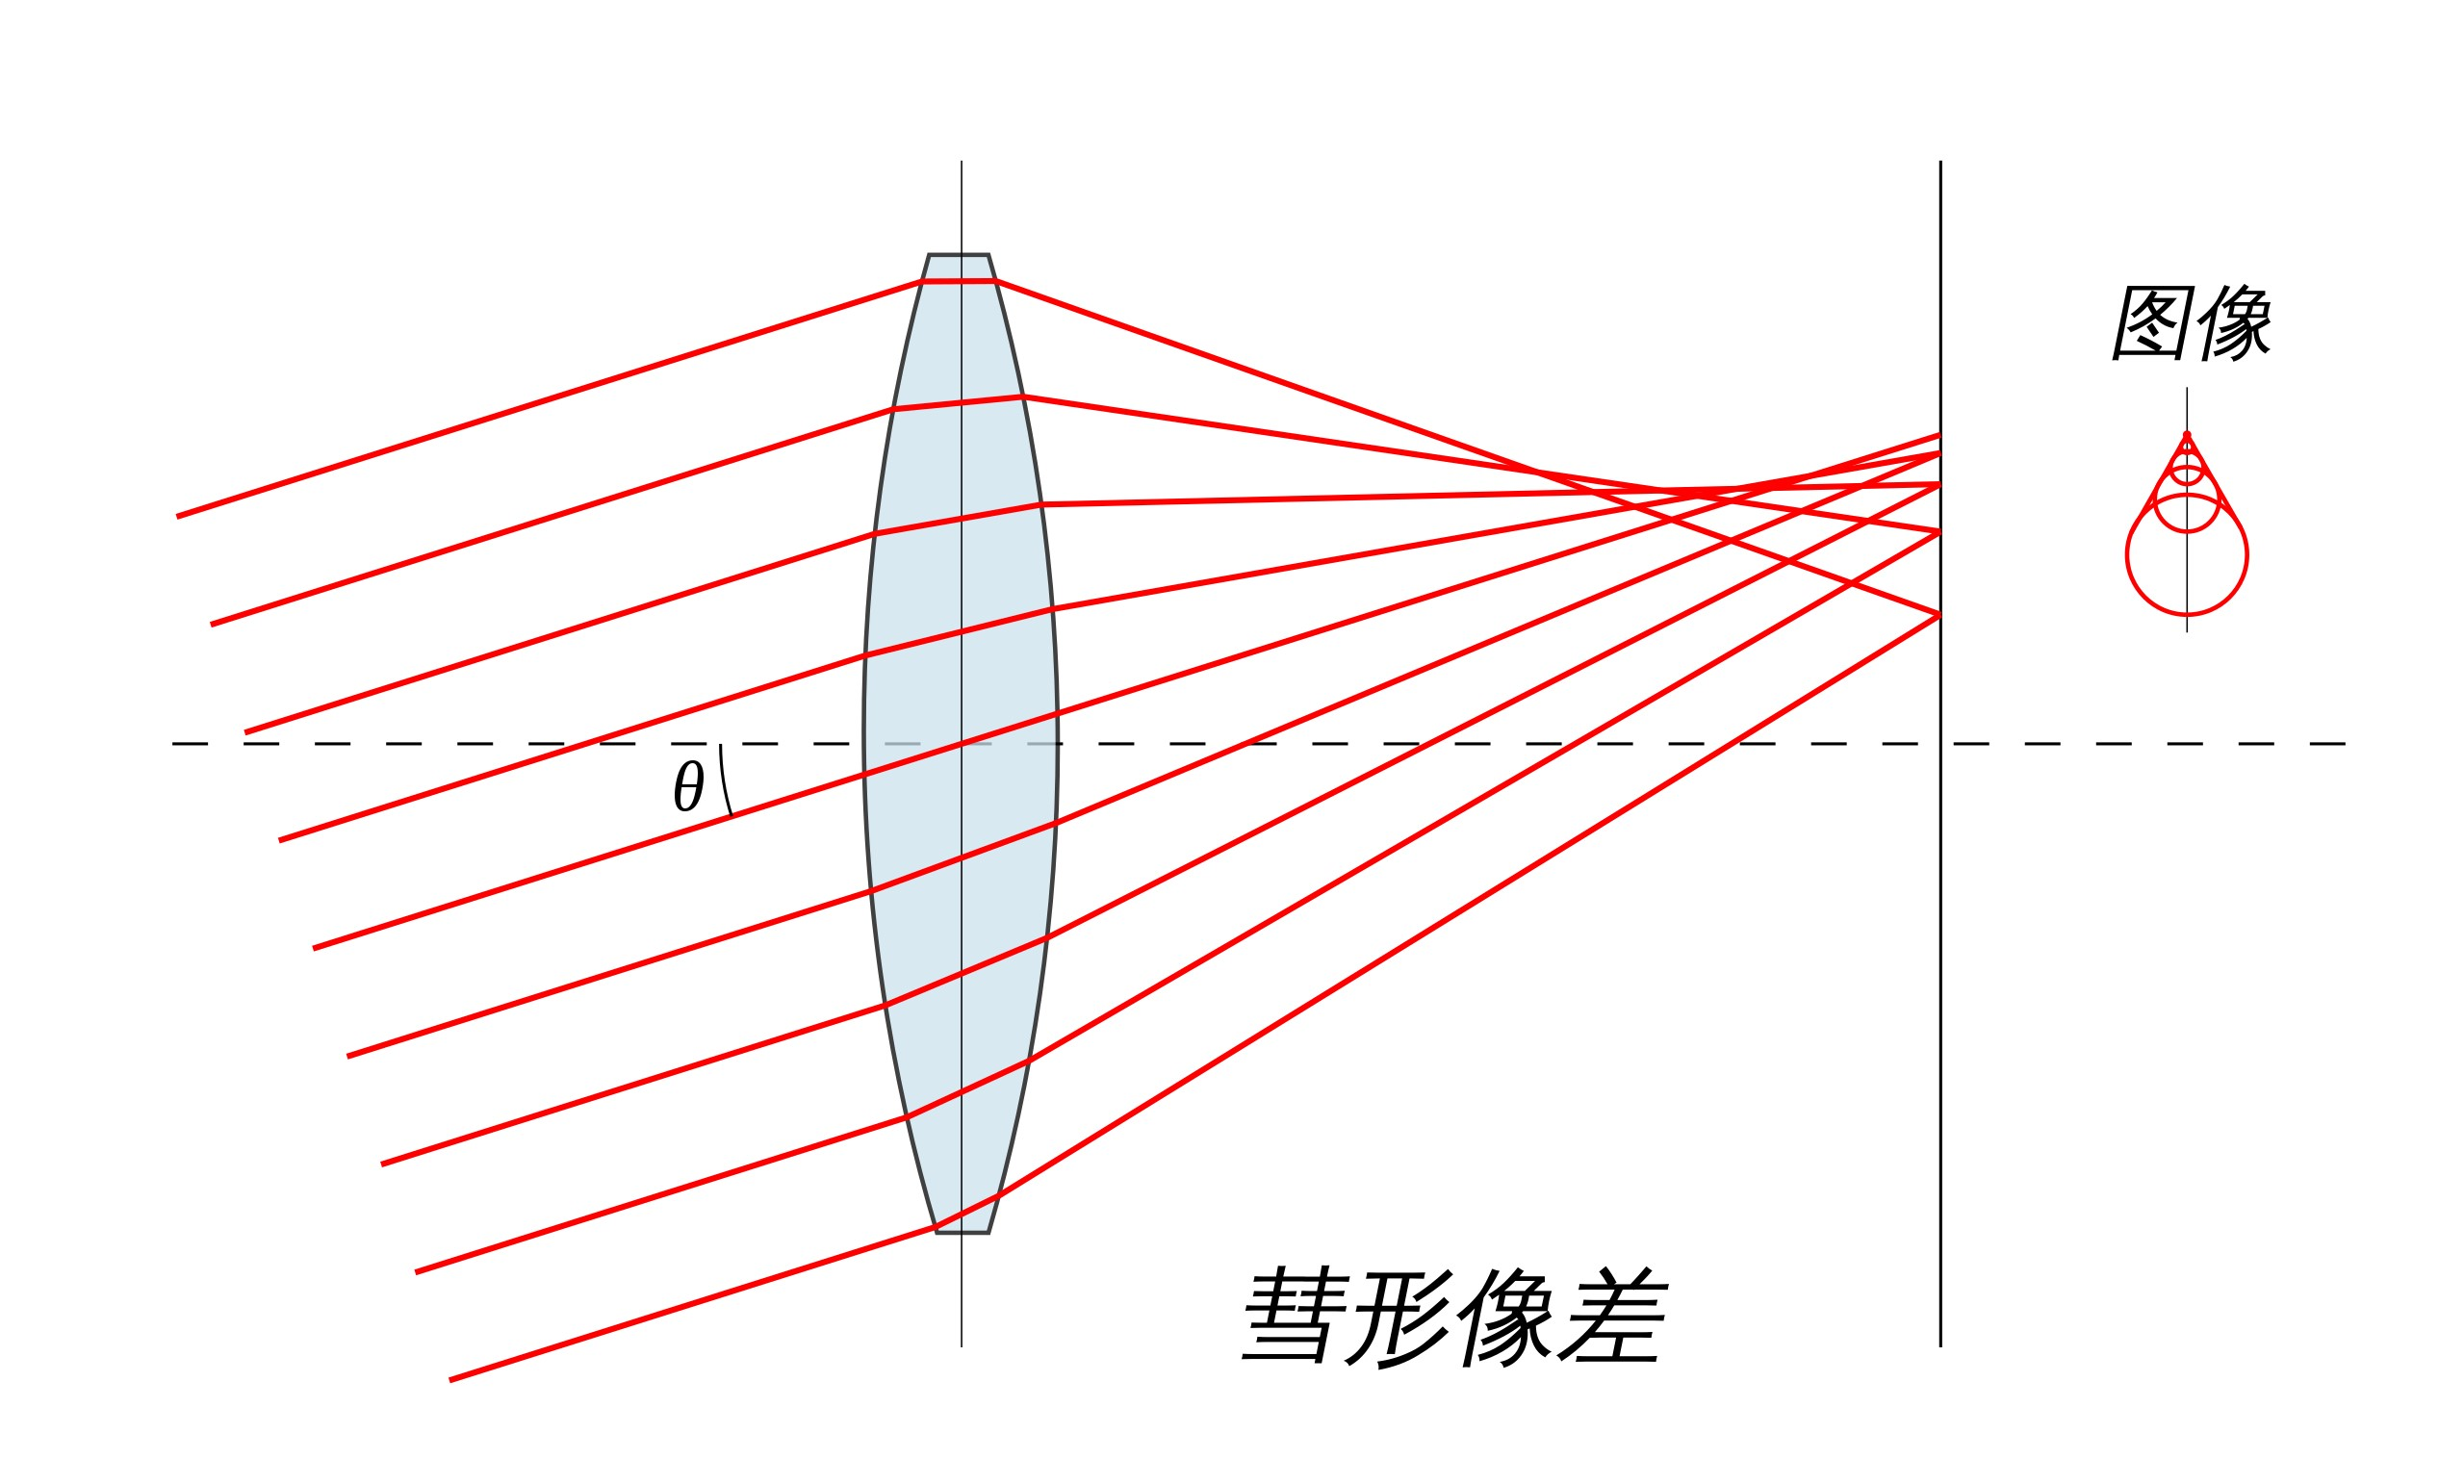
\includegraphics[width=0.5\textwidth]{Lab2_4Gra1.jpg}
			\caption{光学慧差}
			\label{fig:fig1}
		\end{figure}
		
		具体来说,慧差(spherical aberration)是由透镜或反射镜的球面形状导致的光线偏折,使得不同位置的光线聚焦于不同的焦点,导致成像模糊。理想透镜下,来自物体上任意一点的光线会通过透镜在像平面上的单一点聚焦。但是,即便是完美制造的透镜也无法实现这一点,这些偏离理想透镜性能的情况被称为透镜的像差。
		
		\item 关于光学像差的原理补充
		
		像差理论是光学设计求解光学系统初始结构的理论基础。在建立起理想光学系统后,将实际光学系统所成的像偏离理想光学系统的误差称为几何像差,简称像差。光学设计者将几何像差分为七种,即球差、慧差、像散、场曲、畸变、位置色差和倍率色差。产生像差的原因有三点:
		\begin{itemize}
			\item 光线计算公式的非线性;
			\item 物面为平面,折(反)射面为球面(曲面),成像面为曲面;
			\item 不同颜色(波长)的光在折射介质中的折射率不同。
		\end{itemize}
		
		下面简单总结七中光学像差:
		
		\textbf{球差 (Spherical Aberration)}
		
		球差发生在光轴上的物点发出的光束通过光学系统后,不同孔径的光线与光轴交点不同,导致像点位置不一致。这主要是因为物面为平面,而折射面为球面(曲面),导致不同孔径光线在光轴上的焦点相对于理想像点的距离不同。球差的存在会影响成像的清晰度和分辨率。
		
		\textbf{慧差 (Coma)}
		
		慧差是针对轴外光束而言,当光学系统不满足等晕条件时,近轴点成像光束的对称性被破坏,形成彗星状的弥散斑。慧差与孔径大小和视场位置有关,且既与孔径相关又与视场相关。它会使轴外像点变成彗星状,影响轴外像点的清晰度。
		
		\textbf{像散 (Astigmatism)}
		
		像散发生在视场较大时,除了慧差外,还有像散等像差产生。像散是因为光束的子午焦线和弧矢焦线不在同一位置,导致在理想像面上的弥散斑为一椭圆。像散的存在,必然引起像面弯曲,但即便像散为零,像面也不是平的,而是相切于高斯像面中心的二次抛物面。
		
		\textbf{场曲 (Field Curvature)}
		
		场曲是由于实际光学系统的成像面为曲面(由于折射面一般为球面或非球面造成),与理想成像平面的差异所导致。场曲的存在导致无法同时在一个较大平面上成清晰像,即边缘清晰时中心模糊,反之亦然。
		
		\textbf{畸变 (Distortion)}
		
		畸变是由于主光线的实际角放大率不等于+1时导致的,即像方主光线与理想像点不重合。畸变只改变轴外物点在理想像面的成像位置,导致像的形状产生失真,但不影响像的清晰度。
		
		\textbf{位置色差 (Longitudinal Chromatic Aberration)}
		
		位置色差是因为不同波长的光在介质中的折射率不同,导致不同颜色的光在经过光学系统后与光轴的交点不同,即轴上点两种色光之间成像位置的差异。
		
		\textbf{倍率色差 (Transverse Chromatic Aberration)}
		
		倍率色差是因为光学系统对不同色光具有不同的垂轴放大率,导致轴外物点发出的两种色光的主光线在消单色光像差的高斯像面上的交点高度之差。
		
	\end{enumerate}
	% ---
	
	
	
	% 实验前思考题
	\subsection{实验前思考题}
	
	% 思考题1
	\begin{question}
		慧差与孔径、视场的关系?
	\end{question}
	\begin{enumerate}
		\item 先说明上述三个概念:
		
		\textbf{慧差 (Chromatic Aberration)}
		
		慧差是一种因为镜头或其他光学系统中的材料对不同波长的光折射率不同而产生的像差。这种现象导致不同颜色的光在经过光学系统后无法在同一点汇聚,从而在成像时产生颜色边缘或模糊。慧差主要有两种类型:轴向慧差(longitudinal chromatic aberration,也称为色差)和横向慧差(transverse chromatic aberration,也称为色散)。
		
		\textbf{孔径 (Aperture)}
		
		孔径是指光学系统中用于限制通过系统的光束大小的开口。孔径的大小直接影响到成像质量和光量。一般来说,孔径越大,允许进入的光量越多,成像亮度越高,但同时也会增加光学系统的慧差和其他像差。相反,缩小孔径可以减少像差,提高成像的锐度,但会减少进入相机的光量,影响成像的亮度。
		
		\textbf{视场 (Field of View)}
		
		视场是指光学系统能够观察到的空间区域的范围。它通常由角度来描述,在相机和望远镜等光学设备中尤为重要。视场的大小受到光学系统焦距和传感器尺寸的影响。焦距越短,视场越广阔;焦距越长,视场越狭窄。
		
		\item \textbf{慧差与孔径、视场的关系}
		\begin{enumerate}
			\item 孔径与慧差的关系:
			
			孔径大小直接影响慧差的程度。在一个具有固定焦距的光学系统中,随着孔径增大(即允许通过的光线数量增多),光束的边缘部分与光轴的夹角也增大。因为球面透镜或反射镜对于靠近边缘的光线的聚焦能力较差(与理想的聚焦点有所偏离),所以随着孔径的增大,慧差也随之增加。这意味着图像的模糊程度或失焦将更为严重。
			
			增大孔径可以增加进入光学系统的光量,提高成像亮度,但同时也会增加慧差,特别是横向慧差,因为大孔径允许更多角度不同的光线进入,增加了色散的可能性。通过减小孔径可以在一定程度上减少慧差,但这也会减少成像亮度和景深。
			\item 视场与慧差的关系:
			
			随着视场的增大,即图像边缘的光线入射角度增加,这些光线在透镜或反射镜的边缘部分聚焦,导致了更大的慧差。在广角镜头或具有宽视场的望远镜中,边缘图像的质量下降尤为明显,因为这些光线受到更大的偏折。
			
			视场的广阔通常会增加光学系统边缘部分的慧差,尤其是横向慧差。在广角镜头中,由于需要捕捉更广阔的视场,边缘部分的光线与光轴形成较大的角度,导致更严重的色散现象。
			\item 孔径与视场的共同影响:
			
			慧差的量化可以通过几何光学的公式来描述,其中考虑了光线入射角、透镜曲率半径和折射率。一个简化的慧差表达式考虑了光线的入射高度(从透镜中心到光线入射点的距离),孔径大小和透镜的物理属性。虽然具体的数学模型可能较为复杂,但基本原理是:随着孔径的增大或视场的扩大,慧差引起的图像质量下降。
			
			在设计光学系统时,需要综合考虑孔径和视场的大小,以达到理想的成像质量。孔径的选择不仅会影响慧差的程度,也会影响视场中不同部位的成像质量。同时,为了获得更宽广的视场而设计的光学系统需要特别注意控制边缘部分的慧差。
		\end{enumerate}
	\end{enumerate}
	
	% 思考题2
	\begin{question}
		产生色差原因?列举几种消色差的方法。
	\end{question}
	\begin{enumerate}
		\item \textbf{产生色差原因}
		
		光学色差是镜头或光学系统在成像过程中由于光的折射率与波长相关性导致的一种成像缺陷。当不同波长的光通过同一光学元件时,由于折射率的差异,各种颜色的光线在焦点、方向或大小上产生不同程度的分离,导致成像时出现色彩边缘或模糊,影响成像质量。主要表现为两种类型:
		\begin{enumerate}
			\item \textbf{轴向色差(Longitudinal Chromatic Aberration, LCA)}:不同颜色的光在光轴方向上焦点不一致,导致图像上出现彩色晕轮。这种色差主要出现在图像的高对比度边缘处,例如黑白边界。
			\item \textbf{横向色差(Lateral Chromatic Aberration, LaCA)}:不同颜色的光经过光学系统后,在成像平面上呈现不同的放大率,导致彩色边缘平行于光轴的位置错位。这种色差通常出现在图像的边缘部分。
		\end{enumerate}
		
		\item \textbf{消除色差的方法}
		
		色差是由透镜折射率对不同波长光线的依赖性不同引起的,导致不同颜色的光在透镜中聚焦于不同的点。为了减少色差,可以使用具有不同色散特性材料组成的复合透镜,如消色差双胶合镜(achromatic doublet),这种透镜通常由玻璃和氟化物材料制成,以降低光学色散,实现不同颜色光线的更好聚焦。色差的最小化可以通过使用具有不同折射率和色散的材料组合透镜实现。一个常见的方法是使用消色差透镜或者称为消色差双胶合镜,它由冠玻璃和氟玻璃组成,能够在一定波长范围内减少色差,尽管无法完全校正。进一步增加不同组合的透镜可以进一步提高校正程度,例如使用超消色差透镜或apochromat。此外,衍射光学元件(diffractive optical elements)也可以用来校正色差,它们具有与光学玻璃和塑料的正阿贝数相反的负色散特性。
		
		\begin{enumerate}
			\item 使用低色散材料:选用低色散(Low-Dispersion, LD)或超低色散(Extra-Low Dispersion, ED)材料制造光学元件,可以有效减少光的色散,从而减轻色差。
			\item 光学设计优化:通过优化光学系统的设计,例如使用多片镜头组合,调整镜片的曲率和厚度,可以在设计阶段减少色差的产生。
			\item 非球面镜片:使用非球面镜片可以更精确地控制光线的传播,以减少色差和其他像差。
			\item 复合镜头(Achromatic Lens):通过将不同材料的两个或多个镜片粘合在一起制成复合镜头,以抵消不同颜色光线的色散效应。这种方法常用于制造消色差透镜。
			\item 数字后期处理:在图像或视频被捕捉后,可以通过软件算法识别并修正色差,这是现代数码摄影中常见的处理手段。许多相机和图像编辑软件都内置了色差校正功能。
			\item 光栅校正:在一些专业的光学仪器中,会使用光栅来校正色差,尤其是在高精度的测量仪器和天文望远镜中。
		\end{enumerate}
		
		\item \textbf{相关文献调研}
		\begin{enumerate}
			\item 数字图像处理法:通过分析不显示色差的边缘颜色行为,限制颜色差异信号的范围,以此检测和消除色差(Chung2010)。
			
			\item 特制光学系统:设计并构建了用于校正眼睛平均纵向色差的光学系统,保持相对较宽的视场(Benny2007)。
			
			\item 电子镜法:使用超越式电子镜校正色差,通过特定的磁偏转系统和透镜组合来实现色差校正(Mauck1993)。
			
			\item 使用关键点校正单张图像中的色差:通过匹配每个颜色通道的关键点并对其进行对齐,
			来校正单个照片中的色差(Cecchetto2020)。
			
			\item 假彩色滤波技术:利用假彩色滤波技术过滤掉输入图像色度信号中的假彩色成分,减少色差产生的色彩失真(Chang2013)。
		\end{enumerate}
	\end{enumerate}
	
	% 思考题3
	\begin{question}
		针孔滤波的工作原理。
	\end{question}
	\textbf{针孔滤波}是光学中的一个重要概念,主要应用于成像技术中改善图像质量。其工作原理基于波动光学的基本原理,特别是衍射和干涉现象。以下是针孔滤波的工作原理的详细叙述:
	
	\begin{enumerate}
		\item \textbf{基本概念:}
		\begin{itemize}
			\item \textbf{衍射}:当光波遇到障碍物(如缝隙、孔洞等)时,其传播路径会发生偏离,形成新的波前。这种现象称为衍射。
			\item \textbf{干涉}:当两个或多个波遇合时,它们会相互加强(构造干涉)或相互削弱(破坏性干涉),形成新的波形模式。
			\item \textbf{空间频率}:描述图像中细节大小的一个量度。高空间频率对应于图像中的细小细节,而低空间频率对应于图像中的大尺寸特征。
		\end{itemize}
		
		\item \textbf{针孔滤波的工作原理:}
		\begin{enumerate}
			\item \textbf{衍射限制:}
			\begin{itemize}
				\item 光源发出的光波通过物体时,光波会根据物体的结构发生衍射。
				\item 当这些衍射的光波穿过针孔时,由于针孔的尺寸非常小,它只允许通过中心的一部分光波。
				\item 这意味着,针孔作用下,能够通过的光波主要是与物体的细节相对应的那些空间频率较高的成分。
			\end{itemize}
			
			\item \textbf{干涉和重建:}
			\begin{itemize}
				\item 衍射后的光波通过针孔后,这些光波在针孔另一侧重叠并干涉,形成图像。
				\item 由于针孔滤波去除了一些光波成分,通过的光波主要是高空间频率的成分,因此可以改善图像的对比度和分辨率,尤其是在处理细节丰富的场景时。
			\end{itemize}
			
			\item \textbf{空间滤波:}
			\begin{itemize}
				\item 针孔滤波实际上是一种空间滤波技术,它通过物理方式实现对光波空间频率成分的选择性传递。
				\item 这种滤波方式可以用来减少图像的模糊,提高成像系统的光学性能。
			\end{itemize}
		\end{enumerate}
	\end{enumerate}
	
	\textbf{针孔滤波}也是一种图像处理技术,常用于去除图像中的噪声或进行图像增强。它的工作原理基于空间域滤波的概念,利用邻近像素的值对目标像素进行处理,从而实现对图像的平滑或锐化。针孔滤波特别适用于去除小的噪声点,同时保留图像的主要结构和边缘信息。
	
	\begin{enumerate}
		\item \textbf{滤波器的定义:}
		针孔滤波器通常定义为一个小的、中心对称的矩阵,称为核(Kernel)或掩模(Mask)。这个核决定了滤波器如何对目标像素及其邻域像素进行加权和计算。在针孔滤波中,核的中心通常有一个较大的权值,而周围的权值较小或为零,这样设计是为了模拟通过一个小孔(针孔)观察图像的效果,只有中心的光线可以通过。
		
		\item \textbf{滤波过程:}
		针孔滤波的过程可以分为以下几个步骤:
		\begin{itemize}
			\item \textbf{核的移动:} 滤波器核在图像上逐像素移动。对于图像中的每一个像素,都将核置于以该像素为中心的位置。
			\item \textbf{加权和计算:} 计算核内所有像素的加权和。核中心的像素权重最大,反映了针孔滤波的特性。这个加权和替代了原来核中心位置的像素值。
			\item \textbf{边界处理:} 由于核在图像边缘无法完全覆盖像素,因此需要采取一定的边界处理策略,如复制边缘像素、镜像反射或者忽略边缘。
		\end{itemize}
		
		\item \textbf{噪声去除与图像增强:}
		\begin{itemize}
			\item \textbf{噪声去除:} 通过以上加权和计算,小的噪声点(其像素值与周围像素差异较大)会被平滑掉,因为加权和的计算使得这些点的像素值被邻近的像素值所替代。
			\item \textbf{图像增强:} 虽然针孔滤波主要用于噪声去除,但适当调整核中的权值也可以用于增强图像的边缘和细节,使图像看起来更清晰。
		\end{itemize}
	\end{enumerate}
	
	% ---
	
	
	
	% 实验记录	
	\clearpage
	
	% 顶栏
	\begin{table}
		\renewcommand\arraystretch{1.7}
		\centering
		\begin{tabularx}{\textwidth}{|X|X|X|X|}
			\hline
			专业: & 物理学 & 年级: & 2022级 \\
			\hline
			姓名: & 杨舒云 & 学号: & 22344020\\
			\hline
			室温: &  & 实验地点: &  \\
			\hline
			学生签名:& 杨舒云 & 评分: &\\
			\hline
			实验时间:& 2024// & 教师签名:&\\
			\hline
		\end{tabularx}
	\end{table}
	% ---
	
	% 小标题
	\section{Lab2-4 光学像差实验I  \quad\heiti 实验记录}
	% ---
	
	\subsection{实验内容、步骤、结果及讨论}
	
	\begin{figure}[htbp]
		\centering
		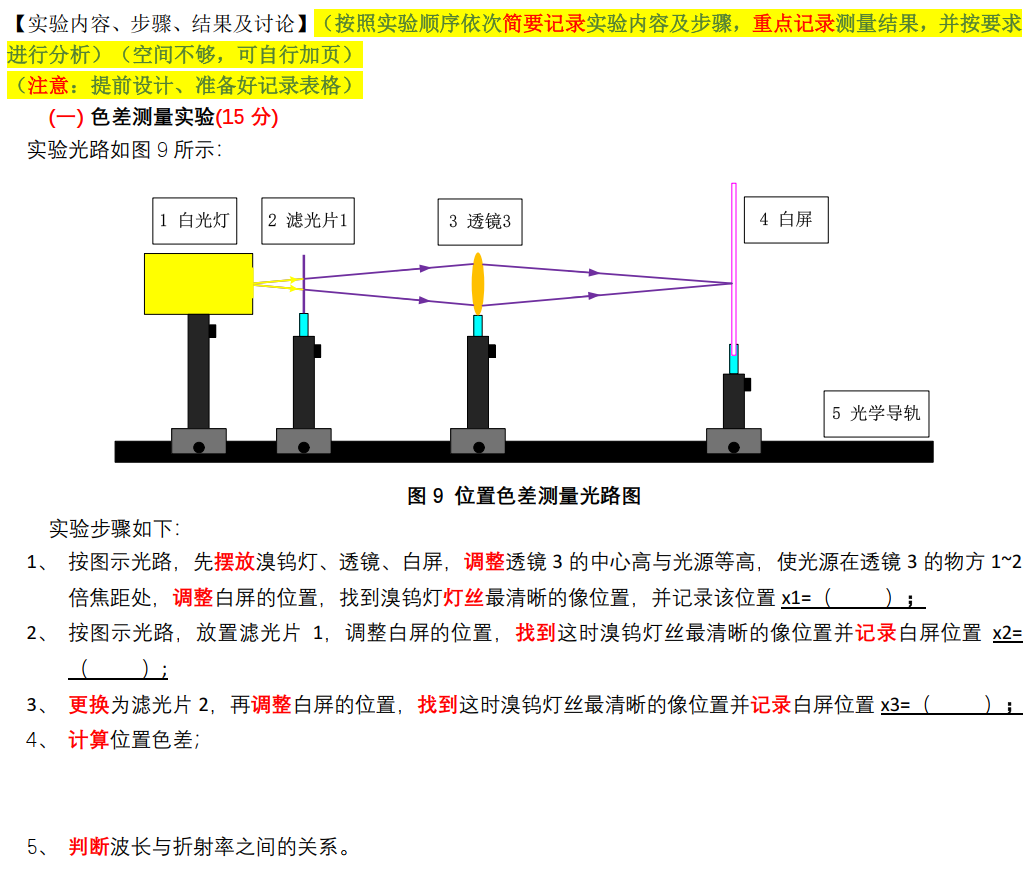
\includegraphics[width=0.8\textwidth]{Lab2_4GraA1.png}
	\end{figure}
	
	
	\clearpage
	\begin{figure}[t]
		\centering
		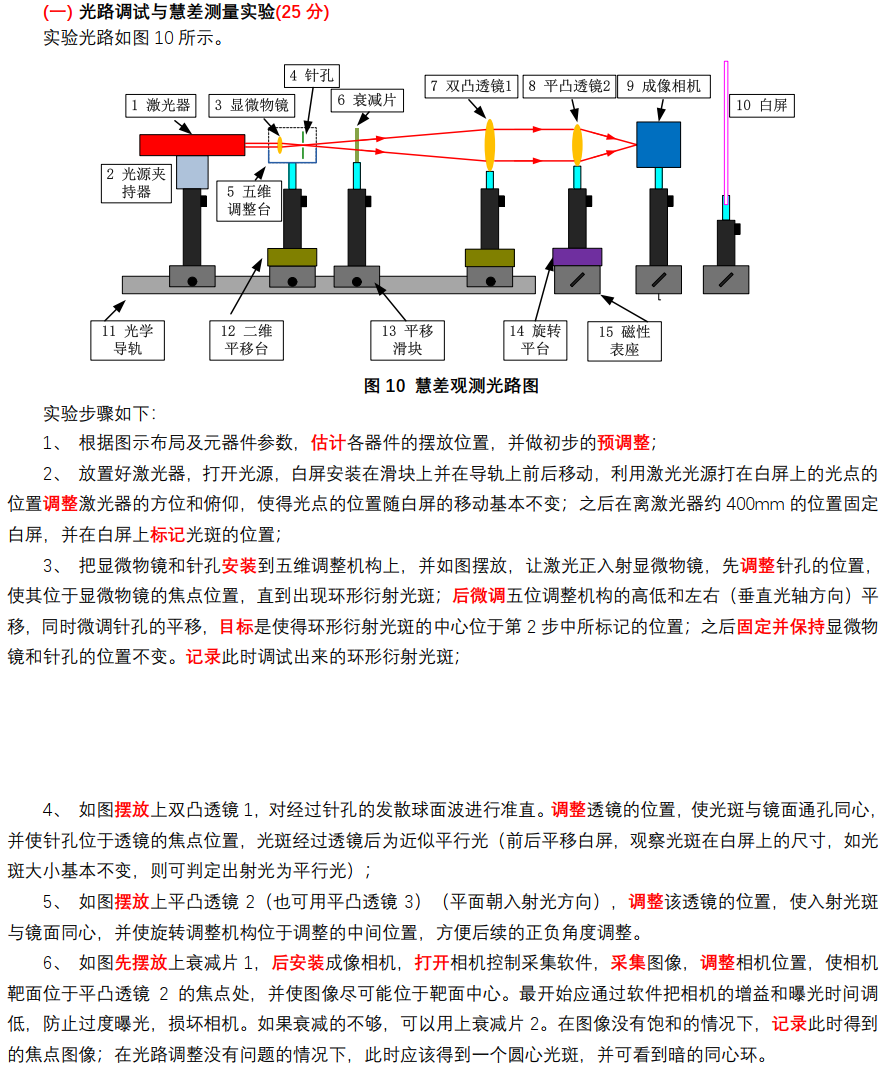
\includegraphics[width=\textwidth]{Lab2_4GraA2.png}
	\end{figure}
	
	\clearpage
	\begin{figure}[t]
		\centering
		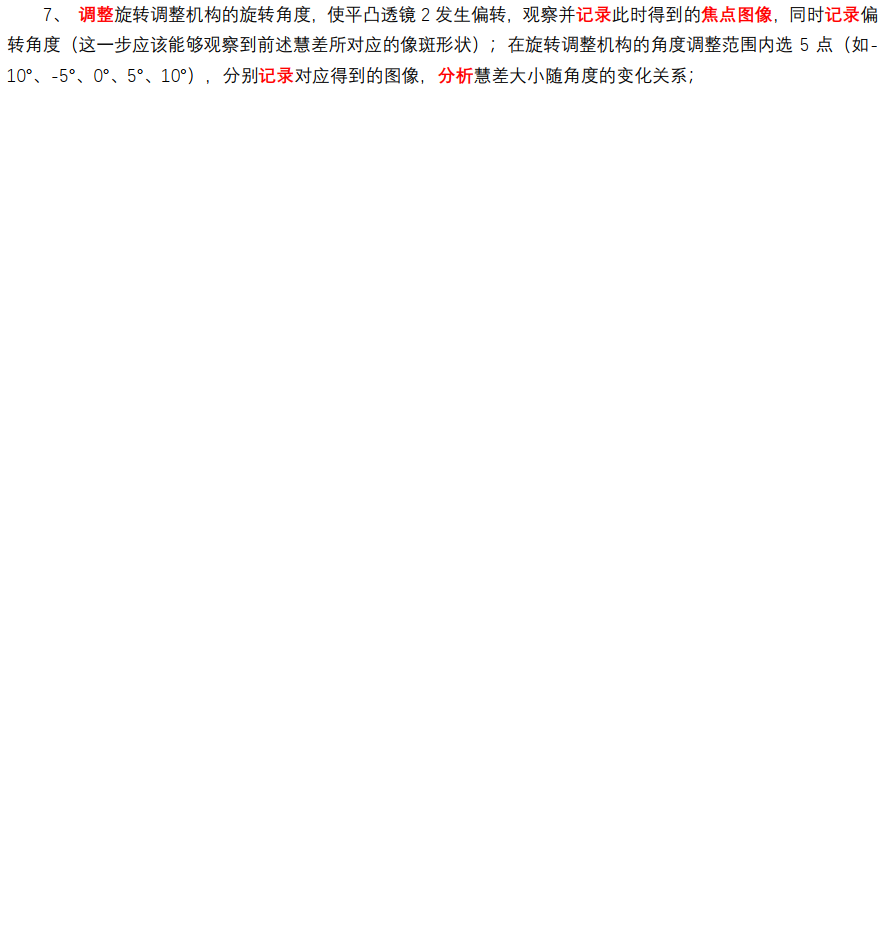
\includegraphics[width=\textwidth]{Lab2_4GraA3.png}
	\end{figure}
	
	\clearpage
	
	\newpage
	
	\null
	
	\newpage
	
	\null
	
	
	
	
	
	
	\newpage
	
	\subsection{实验过程中遇到的问题记录}
	
	\begin{enumerate}
		\item 
		\item 
		\item 
	\end{enumerate}
	\null
	
	
	
	
	
	
	
	
	
	
	
	
	
	
	
	
	% 实验过程记录
	\subsection{实验内容、步骤与结果}
	
	%
	\subsubsection{操作步骤记录}
	\begin{enumerate}
		\item 
	\end{enumerate}	
	
	%
	\subsubsection{}
	\begin{enumerate}
		\item \begin{table}[h]
			\centering
			\caption{表格示例}
			\label{tab:tab1}
			\begin{tabular}{|c|c|c|c|c|c|}
				\hline
				组1/序号i & 1 & 2 & 3 & 4 & 5 \\
				$v_{1i}(m/s)$ & 1.26 & 1.08 & 1.00 & 0.75 & 0.38 \\
				$f_{1i}(Hz)$ & 40073 & 40127 & 40105 & 40088 & 40066 \\
				\hline
				组2/序号i & 1 & 2 & 3 & 4 & 5 \\
				$v_{2i}(m/s)$ & 1.21 & 1.06 & 0.99 & 0.52 & 0.57 \\
				$f_{2i}(Hz)$ & 40143 & 40125 & 40084 & 40080 & 40067 \\
				\hline
				组3/序号i & 1 & 2 & 3 & 4 & 5 \\
				$v_{3i}(m/s)$ & 1.15 & 0.98 & 0.78 & 0.59 & 0.36 \\
				$f_{3i}(Hz)$ & 40135 & 40115 & 40092 & 40070 & 40044 \\
				\hline
			\end{tabular}
		\end{table}		
	\end{enumerate}
	
	% ---
	
	% 原始数据
	\clearpage
	\subsection{原始数据记录}
	实验记录本上的原始数据见%\cref{}(签字)。
	
	实验台桌面整理见%\textbf{附件}部分(\cref{})。
	
	其它原始数据见%\cref{}。
	% ---
	
	% 问题记录
	\subsection{实验过程中遇到的问题记录}
	\begin{enumerate}
		\item 
	\end{enumerate}
	% ---
	
	
	
	% 分析与讨论	
	\clearpage
	
	% 顶栏
	\begin{table}
		\renewcommand\arraystretch{1.7}
		\begin{tabularx}{\textwidth}{|X|X|X|X|}
			\hline
			专业:& 物理学 &年级:& 2022级\\
			\hline
			姓名: & 杨舒云 & 学号:& 22344020\\
			\hline
			日期:& 2024// & 评分: &\\
			\hline
		\end{tabularx}
	\end{table}
	% ---
	
	% 小标题
	\section{XXX 某某某 \quad\heiti 分析与讨论}
	% ---
	
	% 数据处理
	\subsection{实验数据分析}
	
	%
	\subsubsection{}
	\begin{enumerate}
		\item 
	\end{enumerate}
	
	%
	\subsubsection{}
	\begin{enumerate}
		\item 
	\end{enumerate}
	
	%
	\subsubsection{}
	
	% ---
	
	% 实验后思考题
	\subsection{实验后思考题}
	
	%思考题1
	\begin{question}
		
	\end{question}
	
	% 思考题2
	\begin{question}
		
	\end{question}
	
	% 思考题3
	\begin{question}
		
	\end{question}
	
	% ---
	
	
	% 结语部分
	\clearpage
	
	% 小标题
	\section{XXX 某某某 \quad\heiti 结语}
	% ---
	
	% 总结、杂谈与致谢
	\subsection{总结、杂谈与致谢}
	\begin{enumerate}
		\item 
	\end{enumerate}
	% ---
	
	% 参考文献
	\subsection{参考文献}
	[1] 维基百科 https://zh.wikipedia.org
	
	[2] 沈韩.基础物理实验.——北京:科学出版社,2015.2 ISBN:978-7-03-043311-4
	
	% ---
	
	% 附件
	\subsection{附件}
	试验台桌面整理如%\cref{}所示。
	
	实验报告个人签名如\cref{fig:name}。
	
	\begin{figure}[htbp]
		\centering
		
\includegraphics[width=0.7\textwidth]{name.png}
		\caption{个人签名}
		\label{fig:name}
	\end{figure}
	
	% ---
	
	相关代码已上传至Github。
	
	
	
\end{document}